%========================
% Document class and theme
%========================
\documentclass[8pt]{beamer}
\usetheme[progressbar=frametitle]{metropolis}
\setbeamersize{text margin left=10mm, text margin right=10mm}
\usepackage{appendixnumberbeamer} % appendix slide numbering
\setbeamertemplate{theorems}[numbered]

%========================
% Core packages
%========================
\usepackage{amsmath, amsfonts, amssymb, amsthm} % math + theorems
\usepackage{booktabs}        % professional tables
\usepackage{hyperref}        % hyperlinks
\usepackage{xcolor}          % colors
\usepackage{xspace}          % spacing for custom commands

%========================
% Algorithms
%========================
\usepackage{algorithm}
\usepackage{algpseudocode}
\newtheorem{proposition}{Proposition}
\usepackage{bbm}


%========================
% Plots and TikZ
%========================
\usepackage{pgfplots}
\usepgfplotslibrary{dateplot}
\usepackage{tikz}
\usetikzlibrary{positioning}

% ==========================================
% Professional Code Listing Setup
% ==========================================
\usepackage{listings}
\definecolor{codegreen}{rgb}{0,0.6,0}
\definecolor{codegray}{rgb}{0.5,0.5,0.5}
\definecolor{codepurple}{rgb}{0.58,0,0.82}
\definecolor{backcolour}{rgb}{0.95,0.95,0.92}

\lstdefinestyle{mystyle}{
    backgroundcolor=\color{backcolour},   
    commentstyle=\color{codegreen},
    keywordstyle=\color{magenta},
    numberstyle=\tiny\color{codegray},
    stringstyle=\color{codepurple},
    basicstyle=\ttfamily\footnotesize,
    breakatwhitespace=false,         
    breaklines=true,                 
    captionpos=b,                    
    keepspaces=true,                 
    numbers=left,                    
    numbersep=5pt,                  
    showspaces=false,                
    showstringspaces=false,
    showtabs=false,                  
    tabsize=2
}

\lstset{style=mystyle}


%========================
% Custom commands
%========================
\newcommand{\themename}{\textbf{\textsc{metropolis}}\xspace}

%========================
% Custom footline
%========================
\setbeamertemplate{footline}
{%
  \leavevmode%
  \hbox{%
  \begin{beamercolorbox}[wd=.35\paperwidth,ht=2.5ex,dp=1.5ex,center]{author in head/foot}%
    \usebeamerfont{author in head/foot}\insertshortauthor
  \end{beamercolorbox}%
  \begin{beamercolorbox}[wd=.3\paperwidth,ht=2.5ex,dp=1ex,center]{title in head/foot}%
    \usebeamerfont{title in head/foot}\insertshorttitle
  \end{beamercolorbox}%
  \begin{beamercolorbox}[wd=.3\paperwidth,ht=2.5ex,dp=1ex,right]{date in head/foot}%
    \usebeamerfont{date in head/foot}\insertframenumber{} / \inserttotalframenumber
  \end{beamercolorbox}}%
  \vskip0pt%
}

%========================
% Beamer tweaks
%========================
\setbeamertemplate{navigation symbols}{} % remove default navigation symbols


%%%%%%%%%%%%%%%%%%%%%%%%%%%%%%%%%%%%%%%%%%%%%%%%%%%%%%%%%%%%%%%%%%%%
%%%%%%%%%%%%%%%%%%%%%%%%%%%%%%%%%%%%%%%%%%%%%%%%%%%%%%%%%%%%%%%%%%%%
% AQUI SE DEFINEN LAS IMAGENES PARA UTILIZAR DESPUES
%\pgfdeclareimage[interpolate=true, height=7cm,width=16cm]{halton-points}{halton-points}
%\pgfdeclareimage[interpolate=true, height=3cm, width =4cm]
%{serie-petroleo-reducido}{serie-petroleo-reducido}
%\pgfdeclareimage[interpolate=true, height=3cm, width =4cm]{rectangle-triangle}{rectangle-triangle}
%\pgfdeclareimage[interpolate=true, height=3cm, width =4cm]{any-angle}{any-angle}
%\pgfdeclareimage[interpolate=true, height=3cm, width =4cm]{Pythagoras}{Pythagoras}


\title{Chapter 3 - Monte Carlo Methods}
\subtitle{Introduction to Monte Carlo Methods.}
\author{Prof. Alex Alvarez, Ali Raisolsadat}
\institute{School of Mathematical and Computational Sciences \\ University of Prince Edward Island}
\date{} % leave empty or add \today
%\title[Stat 4110]{Stat 4110 Statistical Simulation}
%\subtitle{}
%\author[University of Prince Edward Island]{School of Mathematical and Computational Sciences \\ University of Prince Edward Island}

%========================
% Begin document
%========================
\begin{document}

%-------------------
% Title frame
%-------------------
\maketitle

%-------------------
% Slide 1: Origins of Monte Carlo
%-------------------
\begin{frame}{History of the Monte Carlo Method}
\begin{columns}
    % Left column: history text
    \begin{column}{0.65\textwidth}
        \begin{itemize}
            \item The Monte Carlo method was developed in the 1940s during research for the Manhattan Project.
            \item Mathematician Stanislaw Ulam conceived the idea while recovering from an illness, inspired by thinking about solitaire.
            \item He wondered: \textit{“What is the expected number of winning hands in a game of solitaire?”}
            \item This question led to the use of repeated random sampling to estimate expectations — the foundation of Monte Carlo simulation.
        \end{itemize}
    \end{column}

    % Right column: Ulam picture
    \begin{column}{0.35\textwidth}
        \begin{center}
            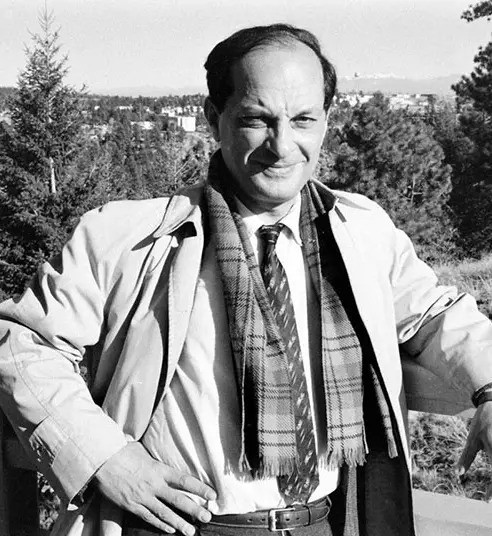
\includegraphics[width=\textwidth]{ulam.jpg} % Replace with actual file
            \\[0.5em]
            \footnotesize Stanislaw Ulam (1909–1984)
        \end{center}
    \end{column}
\end{columns}
\end{frame}

%-------------------
% Slide 2: Early Development
%-------------------
\begin{frame}{Early Development and Implementation}
\begin{columns}
    % Left column: history text
    \begin{column}{0.65\textwidth}
    \begin{itemize}
        \item Ulam proposed using random sampling to solve complex problems in neutron diffusion.
        \item John von Neumann and colleagues formalized the method and implemented it on the ENIAC computer, one of the earliest electronic computers.
        \item The name \textit{“Monte Carlo”} was inspired by the frequent trips of Ulam's uncle to the casino in Monte Carlo, Monaco.
    \end{itemize}
    \end{column}

    % Right column: images
    \begin{column}{0.35\textwidth}
        \begin{center}
        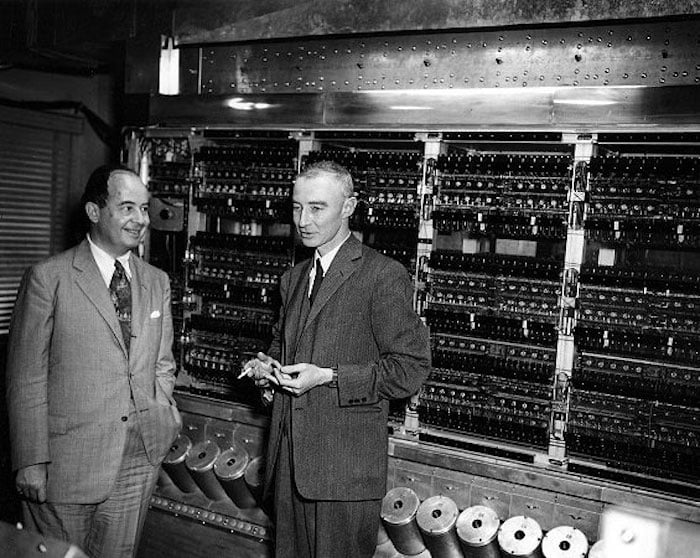
\includegraphics[width=\textwidth]{oppenheimer-neuman-ecp.jpg} % Replace with actual file
        \\[0.5em]
        \footnotesize ENIAC - John von Neumann and Oppenheimer

        \vspace{1em}

        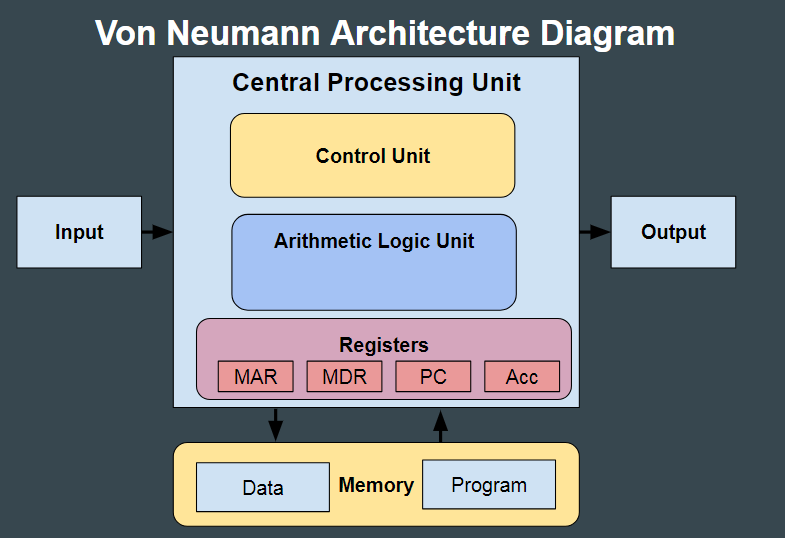
\includegraphics[width=\textwidth]{von-neumann-architecture-gcse-ocr.png} % Replace with actual file
        \\[0.5em]
        \footnotesize Von Neumann architecture
        \end{center}
    \end{column}
\end{columns}
\end{frame}

%-------------------
% Slide 3: Introduction to Monte Carlo Methods
%-------------------
\begin{frame}{Introduction to Monte Carlo Methods}
\begin{itemize}
	\item Monte Carlo methods are a general class of computational algorithms that generate random scenarios to obtain  numerical results.
    \item These methods are widely used in statistical physics, computational chemistry, statistical inference, genetics, and finance.
    \item The Metropolis algorithm, a key Monte Carlo technique, was named one of the top algorithms of the 20th century by a committee of mathematicians, computer scientists, and physicists.
    \item The increasing availability of computational power has greatly expanded the use of Monte Carlo simulations.
    \item Monte Carlo methods can be used to solve a variety of mathematical problems. \textbf{In its most basic form, we use it as a numerical integration method} for integrals with no explicit solution. In this course we will also explore other uses of Monte Carlo methods.
\end{itemize}
\end{frame}

%-------------------
% Slide 4: Particle in Random Medium
%-------------------
\begin{frame}[fragile]{Motivation: Particle in a Random Medium}
\begin{itemize}
    \item Consider a particle $(X_t)_{t=1,2,\dots}$ moving in space $\Omega = \mathbb{R}^d$ according to a stochastic model (e.g., random walk, diffusion, or Markov chain). Randomness may arise from the environment ("medium") or from the particle's motion.
    \item \textbf{Absorption rule:} At each time step $t$, the particle can be absorbed with probability $1 - G(X_t)$, where $G: \Omega \to [0,1]$ is the \textbf{survival weight} at location $X_t$.
    \begin{itemize}
        \item $G(x) \approx 1$: safe location (low absorption risk)
        \item $G(x) \approx 0$: high absorption risk (almost surely absorbed)
    \end{itemize}
    \item The survival probability up to time $T$ is
    \begin{equation*}
        \mathbb{P}(\text{not absorbed at time } T) 
        = \mathbb{E}\Big[ \prod_{t=1}^{T} G(X_t) \Big].
    \end{equation*}
\end{itemize}
\end{frame}

%-------------------
% Slide 5: Multiple Particles
%-------------------
\begin{frame}[fragile]{Multiple Particles in a Random Medium}
\begin{itemize}
    \item Suppose we have $n$ independent particles, each evolving over $T$ time steps according to the stochastic model.
    \item Let $X_{i,t}$ denote the position of particle $i$ at time $t$, for $i = 1,\dots,n$ and $t = 1,\dots,T$.
    \item Let $G(X_{i,t})$ denote the survival weight at that position.
    \item The joint survival probability for all particles is
    \begin{equation*}
        \mathbb{P}(\text{all particles survive up to } T)
        = \mathbb{E}\Big[ \prod_{i=1}^{n} \prod_{t=1}^{T} G(X_{i,t}) \Big].
    \end{equation*}
    \item For continuous positions, this is a $(n \cdot T)$-dimensional integral:
    \begin{align*}
        \mathbb{E}\Big[ \prod_{i=1}^{n} \prod_{t=1}^{T} G(X_{i,t}) \Big] 
        = \int \cdots \int \prod_{i=1}^{n} \prod_{t=1}^{T} G(x_{i,t})
        \, p(x_{1,1},\dots,x_{n,T}) \, dx_{1,1} \cdots dx_{n,T}
    \end{align*}
    where $p(\cdot)$ is the joint density of all particle positions.
\end{itemize}
\end{frame}

%-------------------
% Slide 6: Computing Expected Values
%-------------------
\begin{frame}{Computing Expected Values}
Let $X=(X_1,X_2,\ldots,X_d)$ be a random vector with joint density $f(x_1,x_2,\ldots,x_d)$ and $g: \mathbb{R}^d \rightarrow \mathbb{R}$. We want to compute:
\begin{equation*}
    E g(X)= \int_{\mathbb{R}^d} g(x)f(x) dx
\end{equation*}

If the integral on the right hand side cannot be solved explicitly, we are only left with numerical methods to get an approximated value of that integral. 

\vspace{3mm}

To simplify the presentation we will assume next that we are in the one-dimensional case ($d=1$) but most results apply also in the multidimensional case.
\end{frame}

%-------------------
% Slide 7: The Law of Large Numbers
%-------------------
\begin{frame}{The Law of Large Numbers (LLN)}
\textbf{Theoretical Foundation of Monte Carlo Methods}

\vspace{2mm}

The Monte Carlo method relies on the \textbf{Law of Large Numbers (LLN)}, which ensures that empirical averages converge to their expected values as the sample size grows.

\vspace{2mm}

\textbf{Theorem (Strong Law of Large Numbers):}
Let $(X_i)_{i=1}^\infty$ be a sequence of independent and identically distributed (i.i.d.) random variables with
\begin{equation*}
\mathbb{E}[X_i] = \mu, \quad \mathrm{Var}(X_i) = \sigma^2 < \infty
\end{equation*}
Then, as $n \to \infty$,
\begin{equation*}
\overline{X}_n = \frac{1}{n} \sum_{i=1}^{n} X_i \;\xrightarrow{\text{a.s.}}\; \mu
\end{equation*}
i.e., the sample mean converges almost surely to the true mean.
\end{frame}

%-------------------
% Slide 8: Consequences of the LLN
%-------------------
\begin{frame}{Consequences of the Law of Large Numbers}
\begin{itemize}
  \item Suppose $X_1, X_2, \ldots, X_n$ is a simulated random sample from a random variable $X$ with probability density function $f(x)$.
  \item Then, by the Law of Large Numbers,
  \begin{equation*}
  	\frac{1}{n} \sum_{j=1}^{n} g(X_j) \;\approx\; \mathbb{E}[g(X)] \;=\; \int_{\mathbb{R}} g(x)\, f(x)\, dx
  \end{equation*}
  provided $n$ is large.
  \item In particular, if $U_1, U_2, \ldots, U_n$ are independent random variables uniformly distributed on $[0,1]$, then
  \begin{equation*}
  	\frac{1}{n} \sum_{j=1}^{n} g(U_j) \;\approx\; \mathbb{E}[g(U)] \;=\; \int_{0}^{1} g(x)\, dx
  \end{equation*}  
\end{itemize}
\end{frame}

%-------------------
% Slide 9: Monte Carlo Integration Example
%-------------------
\begin{frame}[fragile]{Monte Carlo Integration Example} 
\textbf{Example}: Compute by Monte Carlo integration $\displaystyle{\int_0^{\pi} \sin x dx}$.

\vspace{3mm}

\textbf{Solution}: Make the change of variable $\displaystyle{y=\frac{1}{\pi}x}$, then:
\begin{equation*}
    \int_0^{\pi} \sin x dx= \pi \int_0^{1} \sin (\pi y) dy
\end{equation*}
   
\begin{algorithm}[H]
\caption{Monte Carlo Estimation of $\displaystyle \pi \int_0^1 \sin(\pi x)\,dx$}
\label{alg:monte-carlo-sine}
\begin{algorithmic}[1]
  \State \textbf{Input:} Number of samples $n$
  \State Generate independent random variables $U_1, U_2, \ldots, U_n \sim \text{Uniform}(0,1)$
  \State Compute the empirical mean:
  \begin{equation*}
  	\widehat{I}_n = \pi \frac{1}{n} \sum_{j=1}^{n} \sin(\pi U_j)
  \end{equation*}
  \State \textbf{Output:} Monte Carlo estimate $\widehat{I}_n$ of the integral
\end{algorithmic}
\end{algorithm}
\end{frame}

%-------------------
% Slide 10: Monte Carlo Integration Example
%-------------------
\begin{frame}[fragile]{Monte Carlo Integration Example}
\textbf{Example}: Compute by Monte Carlo integration 
\begin{equation*}
	\int_0^1 \int_0^1 \sqrt{x+y} e^{xy} dxdy
\end{equation*}

\begin{algorithm}[H]
\caption{Monte Carlo Estimator for $\mathbb{E}\!\left[\sqrt{U+V}\, e^{UV}\right]$}
\begin{algorithmic}[1]
  \State \textbf{Input:} Number of samples $n$
  \State \textbf{Generate} $U_1, U_2, \ldots, U_n \sim \text{Uniform}(0,1)$
  \State \textbf{Generate} $V_1, V_2, \ldots, V_n \sim \text{Uniform}(0,1)$
  \State \textbf{Compute:}
  \begin{equation*}
	\text{Empirical Mean} = \frac{1}{n} \sum_{j=1}^{n} \sqrt{U_j + V_j}\, e^{U_j V_j}
  \end{equation*}
  \State \textbf{Output:} Estimated value of $\mathbb{E}\!\left[\sqrt{U+V}\, e^{UV}\right]$
\end{algorithmic}
\end{algorithm}
\end{frame}

%-------------------
% Slide 11: Homework
%-------------------
\begin{frame}{Homework}
\begin{enumerate}
	\item Compute using a Monte Carlo method $E\left[Z^{2/3}(|Z|+1)\right]$ where $Z$ is a standard normal random variable.
	\item Compute by Monte Carlo integration 
\begin{equation*}
	\int_0^1 \int_0^2 (x+2y) \ln (3x+2y+1) dx dy
\end{equation*}
\textbf{Hint}: First make a change of variable so that the region of integration is the square $[0,1]\times[0,1]$
\end{enumerate}
\end{frame}

\end{document}